\documentclass[]{article}
\usepackage{lmodern}
\usepackage{amssymb,amsmath}
\usepackage{ifxetex,ifluatex}
\usepackage{fixltx2e} % provides \textsubscript
\ifnum 0\ifxetex 1\fi\ifluatex 1\fi=0 % if pdftex
  \usepackage[T1]{fontenc}
  \usepackage[utf8]{inputenc}
\else % if luatex or xelatex
  \ifxetex
    \usepackage{mathspec}
  \else
    \usepackage{fontspec}
  \fi
  \defaultfontfeatures{Ligatures=TeX,Scale=MatchLowercase}
\fi
% use upquote if available, for straight quotes in verbatim environments
\IfFileExists{upquote.sty}{\usepackage{upquote}}{}
% use microtype if available
\IfFileExists{microtype.sty}{%
\usepackage{microtype}
\UseMicrotypeSet[protrusion]{basicmath} % disable protrusion for tt fonts
}{}
\usepackage[margin=1in]{geometry}
\usepackage{hyperref}
\hypersetup{unicode=true,
            pdftitle={CoMM: a collaborative mixed model to dissecting genetic contributions to complex traits by leveraging regulatory information},
            pdfauthor={Jin Liu},
            pdfborder={0 0 0},
            breaklinks=true}
\urlstyle{same}  % don't use monospace font for urls
\usepackage{color}
\usepackage{fancyvrb}
\newcommand{\VerbBar}{|}
\newcommand{\VERB}{\Verb[commandchars=\\\{\}]}
\DefineVerbatimEnvironment{Highlighting}{Verbatim}{commandchars=\\\{\}}
% Add ',fontsize=\small' for more characters per line
\usepackage{framed}
\definecolor{shadecolor}{RGB}{248,248,248}
\newenvironment{Shaded}{\begin{snugshade}}{\end{snugshade}}
\newcommand{\KeywordTok}[1]{\textcolor[rgb]{0.13,0.29,0.53}{\textbf{#1}}}
\newcommand{\DataTypeTok}[1]{\textcolor[rgb]{0.13,0.29,0.53}{#1}}
\newcommand{\DecValTok}[1]{\textcolor[rgb]{0.00,0.00,0.81}{#1}}
\newcommand{\BaseNTok}[1]{\textcolor[rgb]{0.00,0.00,0.81}{#1}}
\newcommand{\FloatTok}[1]{\textcolor[rgb]{0.00,0.00,0.81}{#1}}
\newcommand{\ConstantTok}[1]{\textcolor[rgb]{0.00,0.00,0.00}{#1}}
\newcommand{\CharTok}[1]{\textcolor[rgb]{0.31,0.60,0.02}{#1}}
\newcommand{\SpecialCharTok}[1]{\textcolor[rgb]{0.00,0.00,0.00}{#1}}
\newcommand{\StringTok}[1]{\textcolor[rgb]{0.31,0.60,0.02}{#1}}
\newcommand{\VerbatimStringTok}[1]{\textcolor[rgb]{0.31,0.60,0.02}{#1}}
\newcommand{\SpecialStringTok}[1]{\textcolor[rgb]{0.31,0.60,0.02}{#1}}
\newcommand{\ImportTok}[1]{#1}
\newcommand{\CommentTok}[1]{\textcolor[rgb]{0.56,0.35,0.01}{\textit{#1}}}
\newcommand{\DocumentationTok}[1]{\textcolor[rgb]{0.56,0.35,0.01}{\textbf{\textit{#1}}}}
\newcommand{\AnnotationTok}[1]{\textcolor[rgb]{0.56,0.35,0.01}{\textbf{\textit{#1}}}}
\newcommand{\CommentVarTok}[1]{\textcolor[rgb]{0.56,0.35,0.01}{\textbf{\textit{#1}}}}
\newcommand{\OtherTok}[1]{\textcolor[rgb]{0.56,0.35,0.01}{#1}}
\newcommand{\FunctionTok}[1]{\textcolor[rgb]{0.00,0.00,0.00}{#1}}
\newcommand{\VariableTok}[1]{\textcolor[rgb]{0.00,0.00,0.00}{#1}}
\newcommand{\ControlFlowTok}[1]{\textcolor[rgb]{0.13,0.29,0.53}{\textbf{#1}}}
\newcommand{\OperatorTok}[1]{\textcolor[rgb]{0.81,0.36,0.00}{\textbf{#1}}}
\newcommand{\BuiltInTok}[1]{#1}
\newcommand{\ExtensionTok}[1]{#1}
\newcommand{\PreprocessorTok}[1]{\textcolor[rgb]{0.56,0.35,0.01}{\textit{#1}}}
\newcommand{\AttributeTok}[1]{\textcolor[rgb]{0.77,0.63,0.00}{#1}}
\newcommand{\RegionMarkerTok}[1]{#1}
\newcommand{\InformationTok}[1]{\textcolor[rgb]{0.56,0.35,0.01}{\textbf{\textit{#1}}}}
\newcommand{\WarningTok}[1]{\textcolor[rgb]{0.56,0.35,0.01}{\textbf{\textit{#1}}}}
\newcommand{\AlertTok}[1]{\textcolor[rgb]{0.94,0.16,0.16}{#1}}
\newcommand{\ErrorTok}[1]{\textcolor[rgb]{0.64,0.00,0.00}{\textbf{#1}}}
\newcommand{\NormalTok}[1]{#1}
\usepackage{longtable,booktabs}
\usepackage{graphicx,grffile}
\makeatletter
\def\maxwidth{\ifdim\Gin@nat@width>\linewidth\linewidth\else\Gin@nat@width\fi}
\def\maxheight{\ifdim\Gin@nat@height>\textheight\textheight\else\Gin@nat@height\fi}
\makeatother
% Scale images if necessary, so that they will not overflow the page
% margins by default, and it is still possible to overwrite the defaults
% using explicit options in \includegraphics[width, height, ...]{}
\setkeys{Gin}{width=\maxwidth,height=\maxheight,keepaspectratio}
\IfFileExists{parskip.sty}{%
\usepackage{parskip}
}{% else
\setlength{\parindent}{0pt}
\setlength{\parskip}{6pt plus 2pt minus 1pt}
}
\setlength{\emergencystretch}{3em}  % prevent overfull lines
\providecommand{\tightlist}{%
  \setlength{\itemsep}{0pt}\setlength{\parskip}{0pt}}
\setcounter{secnumdepth}{0}
% Redefines (sub)paragraphs to behave more like sections
\ifx\paragraph\undefined\else
\let\oldparagraph\paragraph
\renewcommand{\paragraph}[1]{\oldparagraph{#1}\mbox{}}
\fi
\ifx\subparagraph\undefined\else
\let\oldsubparagraph\subparagraph
\renewcommand{\subparagraph}[1]{\oldsubparagraph{#1}\mbox{}}
\fi

%%% Use protect on footnotes to avoid problems with footnotes in titles
\let\rmarkdownfootnote\footnote%
\def\footnote{\protect\rmarkdownfootnote}

%%% Change title format to be more compact
\usepackage{titling}

% Create subtitle command for use in maketitle
\providecommand{\subtitle}[1]{
  \posttitle{
    \begin{center}\large#1\end{center}
    }
}

\setlength{\droptitle}{-2em}

  \title{CoMM: a collaborative mixed model to dissecting genetic contributions to
complex traits by leveraging regulatory information}
    \pretitle{\vspace{\droptitle}\centering\huge}
  \posttitle{\par}
    \author{Jin Liu}
    \preauthor{\centering\large\emph}
  \postauthor{\par}
      \predate{\centering\large\emph}
  \postdate{\par}
    \date{2019-04-12}


\begin{document}
\maketitle

\subsubsection{Introduction}\label{introduction}

This vignette provides an introduction to the \texttt{CoMM} package. R
package \texttt{CoMM} implements CoMM, a collaborative mixed model to
dissecting genetic contributions to complex traits by leveraging
regulatory information. The package can be installed with the command:

\texttt{library(devtools)}

\texttt{install\_github("gordonliu810822/CoMM")}

The package can be loaded with the command:

\begin{Shaded}
\begin{Highlighting}[]
\KeywordTok{library}\NormalTok{(}\StringTok{"CoMM"}\NormalTok{)}
\end{Highlighting}
\end{Shaded}

\subsubsection{Fit CoMM using simulated
data}\label{fit-comm-using-simulated-data}

We first generate genotype data using function \emph{genRawGeno}:

\begin{Shaded}
\begin{Highlighting}[]
\KeywordTok{library}\NormalTok{(mvtnorm)}
\NormalTok{L =}\StringTok{ }\DecValTok{1}\NormalTok{; M =}\StringTok{ }\DecValTok{100}\NormalTok{; rho =}\FloatTok{0.5}
\NormalTok{n1 =}\StringTok{ }\DecValTok{350}\NormalTok{; n2 =}\StringTok{ }\DecValTok{5000}\NormalTok{;}
\NormalTok{maf =}\StringTok{ }\KeywordTok{runif}\NormalTok{(M,}\FloatTok{0.05}\NormalTok{,}\FloatTok{0.5}\NormalTok{)}
\NormalTok{X =}\StringTok{ }\KeywordTok{genRawGeno}\NormalTok{(maf, L, M, rho, n1 }\OperatorTok{+}\StringTok{ }\NormalTok{n2);}
\end{Highlighting}
\end{Shaded}

Then, effect sizes are generated from standard Gaussian distribution
with sparse structure:

\begin{Shaded}
\begin{Highlighting}[]
\NormalTok{beta_prop =}\StringTok{ }\FloatTok{0.2}\NormalTok{;}
\NormalTok{b =}\StringTok{ }\KeywordTok{numeric}\NormalTok{(M);}
\NormalTok{m =}\StringTok{ }\NormalTok{M }\OperatorTok{*}\StringTok{ }\NormalTok{beta_prop;}
\NormalTok{b[}\KeywordTok{sample}\NormalTok{(M,m)] =}\StringTok{ }\KeywordTok{rnorm}\NormalTok{(m);}
\end{Highlighting}
\end{Shaded}

Subsequently, the gene expression \texttt{y} is generated by controlling
cellular heritability at prespecified level (\texttt{h2y}):

\begin{Shaded}
\begin{Highlighting}[]
\NormalTok{h2y =}\StringTok{ }\FloatTok{0.05}\NormalTok{;}
\NormalTok{b0 =}\StringTok{ }\DecValTok{6}\NormalTok{;}
\NormalTok{y0 <-}\StringTok{ }\NormalTok{X}\OperatorTok\NormalTok{b }\OperatorTok{+}\StringTok{ }\NormalTok{b0;}
\NormalTok{y  <-}\StringTok{ }\NormalTok{y0 }\OperatorTok{+}\StringTok{ }\NormalTok{(}\KeywordTok{as.vector}\NormalTok{(}\KeywordTok{var}\NormalTok{(y0)}\OperatorTok{*}\NormalTok{(}\DecValTok{1}\OperatorTok{-}\NormalTok{h2y)}\OperatorTok{/}\NormalTok{h2y))}\OperatorTok{^}\FloatTok{0.5}\OperatorTok{*}\KeywordTok{rnorm}\NormalTok{(n1}\OperatorTok{+}\NormalTok{n2);}
\end{Highlighting}
\end{Shaded}

Finally, the phenotype data is generated as the generative model of CoMM
with a prespecified trait heritability (\texttt{h2}) as:

\begin{Shaded}
\begin{Highlighting}[]
\NormalTok{h2 =}\StringTok{ }\FloatTok{0.001}\NormalTok{;}
\NormalTok{y1 <-}\StringTok{ }\NormalTok{y[}\DecValTok{1}\OperatorTok{:}\NormalTok{n1]}
\NormalTok{X1 <-}\StringTok{ }\NormalTok{X[}\DecValTok{1}\OperatorTok{:}\NormalTok{n1,]}
\NormalTok{y2 <-}\StringTok{ }\NormalTok{y0[(n1}\OperatorTok{+}\DecValTok{1}\NormalTok{)}\OperatorTok{:}\NormalTok{(n1}\OperatorTok{+}\NormalTok{n2)]}
\NormalTok{X2 <-}\StringTok{ }\NormalTok{X[(n1}\OperatorTok{+}\DecValTok{1}\NormalTok{)}\OperatorTok{:}\NormalTok{(n1}\OperatorTok{+}\NormalTok{n2),]}
\NormalTok{alpha0 <-}\StringTok{ }\DecValTok{3}  
\NormalTok{alpha <-}\StringTok{ }\FloatTok{0.3}
\NormalTok{sz2 <-}\StringTok{ }\KeywordTok{var}\NormalTok{(y2}\OperatorTok{*}\NormalTok{alpha) }\OperatorTok{*}\StringTok{ }\NormalTok{((}\DecValTok{1}\OperatorTok{-}\NormalTok{h2)}\OperatorTok{/}\NormalTok{h2)}
\NormalTok{z <-}\StringTok{ }\NormalTok{alpha0 }\OperatorTok{+}\StringTok{ }\NormalTok{y2}\OperatorTok{*}\NormalTok{alpha }\OperatorTok{+}\StringTok{ }\KeywordTok{rnorm}\NormalTok{(n2,}\DecValTok{0}\NormalTok{,}\KeywordTok{sqrt}\NormalTok{(sz2))}
\end{Highlighting}
\end{Shaded}

The genotype data \texttt{X1} and \texttt{X2} are normalized as

\begin{Shaded}
\begin{Highlighting}[]
\NormalTok{y =}\StringTok{ }\NormalTok{y1;}
\NormalTok{mean.x1 =}\StringTok{ }\KeywordTok{apply}\NormalTok{(X1,}\DecValTok{2}\NormalTok{,mean);}
\NormalTok{x1m =}\StringTok{ }\KeywordTok{sweep}\NormalTok{(X1,}\DecValTok{2}\NormalTok{,mean.x1);}
\NormalTok{std.x1 =}\StringTok{ }\KeywordTok{apply}\NormalTok{(x1m,}\DecValTok{2}\NormalTok{,sd)}
\NormalTok{x1p =}\StringTok{ }\KeywordTok{sweep}\NormalTok{(x1m,}\DecValTok{2}\NormalTok{,std.x1,}\StringTok{"/"}\NormalTok{);}
\NormalTok{x1p =}\StringTok{ }\NormalTok{x1p}\OperatorTok{/}\KeywordTok{sqrt}\NormalTok{(}\KeywordTok{dim}\NormalTok{(x1p)[}\DecValTok{2}\NormalTok{])}

\NormalTok{mean.x2 =}\StringTok{ }\KeywordTok{apply}\NormalTok{(X2,}\DecValTok{2}\NormalTok{,mean);}
\NormalTok{x2m =}\StringTok{ }\KeywordTok{sweep}\NormalTok{(X2,}\DecValTok{2}\NormalTok{,mean.x2);}
\NormalTok{std.x2 =}\StringTok{ }\KeywordTok{apply}\NormalTok{(x2m,}\DecValTok{2}\NormalTok{,sd)}
\NormalTok{x2p =}\StringTok{ }\KeywordTok{sweep}\NormalTok{(x2m,}\DecValTok{2}\NormalTok{,std.x2,}\StringTok{"/"}\NormalTok{);}
\NormalTok{x2p =}\StringTok{ }\NormalTok{x2p}\OperatorTok{/}\KeywordTok{sqrt}\NormalTok{(}\KeywordTok{dim}\NormalTok{(x2p)[}\DecValTok{2}\NormalTok{])}

\NormalTok{w2 =}\StringTok{ }\KeywordTok{matrix}\NormalTok{(}\KeywordTok{rep}\NormalTok{(}\DecValTok{1}\NormalTok{,n2),}\DataTypeTok{ncol=}\DecValTok{1}\NormalTok{);}
\NormalTok{w1 =}\StringTok{ }\KeywordTok{matrix}\NormalTok{(}\KeywordTok{rep}\NormalTok{(}\DecValTok{1}\NormalTok{,n1),}\DataTypeTok{ncol=}\DecValTok{1}\NormalTok{);}
\end{Highlighting}
\end{Shaded}

Initilize the parameters by using linear mixed model (function
\emph{lmm\_pxem}, LMM implemented (n \textless{} p) using
\href{https://www.jstor.org/stable/2337481?seq=1\#page_scan_tab_contents}{PX-EM
algorithm}, function \emph{lmm\_pxem2}, LMM implemented (n
\textgreater{} p)):

\begin{Shaded}
\begin{Highlighting}[]
\NormalTok{fm0 =}\StringTok{ }\KeywordTok{lmm_pxem2}\NormalTok{(y, w1,x1p, }\DecValTok{100}\NormalTok{)}
\NormalTok{sigma2beta =fm0}\OperatorTok{$}\NormalTok{sigma2beta;}
\NormalTok{sigma2y =fm0}\OperatorTok{$}\NormalTok{sigma2y;}
\NormalTok{beta0 =}\StringTok{ }\NormalTok{fm0}\OperatorTok{$}\NormalTok{beta0;}
\end{Highlighting}
\end{Shaded}

Fit CoMM w/ and w/o constraint that alpha = 0 as

\begin{Shaded}
\begin{Highlighting}[]
\NormalTok{fmHa =}\StringTok{ }\KeywordTok{CoMM_covar_pxem}\NormalTok{(y, z, x1p, x2p, w1, w2,}\DataTypeTok{constr =} \DecValTok{0}\NormalTok{);}
\NormalTok{fmH0 =}\StringTok{ }\KeywordTok{CoMM_covar_pxem}\NormalTok{(y, z, x1p, x2p, w1, w2,}\DataTypeTok{constr =} \DecValTok{1}\NormalTok{);}
\NormalTok{loglikHa =}\StringTok{ }\KeywordTok{max}\NormalTok{(fmHa}\OperatorTok{$}\NormalTok{loglik,}\DataTypeTok{na.rm=}\NormalTok{T)}
\NormalTok{loglikH0 =}\StringTok{ }\KeywordTok{max}\NormalTok{(fmH0}\OperatorTok{$}\NormalTok{loglik,}\DataTypeTok{na.rm=}\NormalTok{T)}
\NormalTok{tstat =}\StringTok{ }\DecValTok{2} \OperatorTok{*}\StringTok{ }\NormalTok{(loglikHa }\OperatorTok{-}\StringTok{ }\NormalTok{loglikH0);}
\NormalTok{pval =}\StringTok{ }\KeywordTok{pchisq}\NormalTok{(tstat,}\DecValTok{1}\NormalTok{,}\DataTypeTok{lower.tail=}\NormalTok{F)}
\NormalTok{alpha_hat =}\StringTok{ }\NormalTok{fmHa}\OperatorTok{$}\NormalTok{alpha }
\end{Highlighting}
\end{Shaded}

\subsubsection{Fit CoMM using GWAS and eQTL
data}\label{fit-comm-using-gwas-and-eqtl-data}

The example of running CoMM using GWAS and eQTL data in plink binary
format

\begin{Shaded}
\begin{Highlighting}[]
\NormalTok{file1 =}\StringTok{ "1000G.EUR.QC.1"}\NormalTok{;}
\NormalTok{file2 =}\StringTok{ "NFBC_filter_mph10"}\NormalTok{;}
\NormalTok{file3 =}\StringTok{ "Geuvadis_gene_expression_qn.txt"}\NormalTok{;}
\NormalTok{file4 =}\StringTok{ ""}\NormalTok{;}
\NormalTok{file5 =}\StringTok{ "pc5_NFBC_filter_mph10.txt"}\NormalTok{;}
\NormalTok{whichPheno =}\StringTok{ }\DecValTok{1}\NormalTok{;}
\NormalTok{bw =}\StringTok{ }\DecValTok{500000}\NormalTok{;}
\end{Highlighting}
\end{Shaded}

Here, file1 is the prefix for eQTL genotype data in plink binary format,
file2 is the GWAS data in plink binary format, file3 is the gene
expression file with extended name, file4 and file5 are covariates file
for eQTL and GWAS data, respectively. Then run
\texttt{fm\ =\ CoMM\_testing\_run(file1,file2,file3,\ file4,file5,\ whichPheno,\ bw);}.
For gene expresion file, it must have the following format (rows for
genes and columns for individuais and note that it must be tab
delimited):

\begin{longtable}[]{@{}rrlllrrr@{}}
\toprule
lower & up & genetype1 & genetype2 & TargetID & Chr & HG00105 &
HG00115\tabularnewline
\midrule
\endhead
59783540 & 59843484 & lincRNA & PART1 & ENSG00000152931.6 & 5 &
0.5126086 & 0.7089508\tabularnewline
48128225 & 48148330 & protein\_coding & UPP1 & ENSG00000183696.9 & 7 &
1.4118007 & -0.0135644\tabularnewline
57846106 & 57853063 & protein\_coding & INHBE & ENSG00000139269.2 & 12 &
0.5755268 & -1.0162217\tabularnewline
116054583 & 116164515 & protein\_coding & AFAP1L2 & ENSG00000169129.8 &
10 & 1.1117776 & 0.0407033\tabularnewline
22157909 & 22396763 & protein\_coding & RAPGEF5 & ENSG00000136237.12 & 7
& 0.2831573 & -0.1772559\tabularnewline
11700964 & 11743303 & lincRNA & RP11-434C1.1 & ENSG00000247157.2 & 12 &
0.2550282 & -0.2831573\tabularnewline
\bottomrule
\end{longtable}

To make `CoMM' further speeding, we implement multiple thread version of
`CoMM' by just run
\texttt{fm\ =\ CoMM\_testing\_run\_mt(file1,file2,file3,\ file4,file5,\ whichPheno,\ bw,\ coreNum);}
where \texttt{coreNum\ =\ 24} is the number of cores in your CPU.

\subsubsection{Figures}\label{figures}

The following data and codes are used to produce one of the figures in
the Yang et al. (2018).

\begin{Shaded}
\begin{Highlighting}[]
\NormalTok{dat_rej =}\StringTok{ }\NormalTok{dat[[}\DecValTok{3}\NormalTok{]];}
\NormalTok{dat_rej}\OperatorTok{$}\NormalTok{h2z=}\KeywordTok{paste}\NormalTok{(}\StringTok{""}\NormalTok{,dat_rej}\OperatorTok{$}\NormalTok{h2,}\DataTypeTok{sep=}\StringTok{""}\NormalTok{)}
\NormalTok{dat_rej}\OperatorTok{$}\NormalTok{Power =}\StringTok{ }\NormalTok{dat_rej}\OperatorTok{$}\NormalTok{rej_prop}
\NormalTok{dat_rej}\OperatorTok{$}\NormalTok{Sparsity =}\StringTok{ }\NormalTok{dat_rej}\OperatorTok{$}\NormalTok{beta_prop}
\NormalTok{dat_rej}\OperatorTok{$}\NormalTok{sd_rej =}\StringTok{ }\KeywordTok{as.numeric}\NormalTok{(}\KeywordTok{as.character}\NormalTok{(dat_rej}\OperatorTok{$}\NormalTok{sd_rej))}
\NormalTok{dat_rej =}\StringTok{ }\NormalTok{dat_rej[dat_rej}\OperatorTok{$}\NormalTok{Method}\OperatorTok{!=}\StringTok{"2-stage:AUDI"}\NormalTok{,]}
\KeywordTok{library}\NormalTok{(plyr)}
\NormalTok{dat_rej}\OperatorTok{$}\NormalTok{Method=}\KeywordTok{revalue}\NormalTok{(dat_rej}\OperatorTok{$}\NormalTok{Method, }\KeywordTok{c}\NormalTok{(}\StringTok{"AUDI"}\NormalTok{=}\StringTok{"CoMM"}\NormalTok{))}
\NormalTok{dat_rej}\OperatorTok{$}\NormalTok{Method=}\KeywordTok{revalue}\NormalTok{(dat_rej}\OperatorTok{$}\NormalTok{Method, }\KeywordTok{c}\NormalTok{(}\StringTok{"2-stage:Ridge"}\NormalTok{=}\StringTok{"PrediXcan:Ridge"}\NormalTok{))}
\NormalTok{dat_rej}\OperatorTok{$}\NormalTok{Method=}\KeywordTok{revalue}\NormalTok{(dat_rej}\OperatorTok{$}\NormalTok{Method, }\KeywordTok{c}\NormalTok{(}\StringTok{"2-stage:Enet"}\NormalTok{=}\StringTok{"PrediXcan:Enet"}\NormalTok{))}
\NormalTok{dat_rej}\OperatorTok{$}\NormalTok{Method=}\KeywordTok{droplevels}\NormalTok{(dat_rej}\OperatorTok{$}\NormalTok{Method)}

\NormalTok{rho =}\StringTok{ }\FloatTok{0.5}\NormalTok{; n2 =}\StringTok{ }\DecValTok{8000}\NormalTok{;}
\NormalTok{t1e_rej =}\StringTok{ }\NormalTok{dat_rej[dat_rej}\OperatorTok{$}\NormalTok{RhoX}\OperatorTok{==}\NormalTok{rho}\OperatorTok{&}\NormalTok{dat_rej}\OperatorTok{$}\NormalTok{n2}\OperatorTok{==}\NormalTok{n2,]}

\NormalTok{t1e_rej}\OperatorTok{$}\NormalTok{h2z =}\StringTok{ }\KeywordTok{factor}\NormalTok{(t1e_rej}\OperatorTok{$}\NormalTok{h2z)}
\NormalTok{t1e_rej}\OperatorTok{$}\NormalTok{h2y =}\StringTok{ }\KeywordTok{factor}\NormalTok{(t1e_rej}\OperatorTok{$}\NormalTok{h2y)}
\NormalTok{t1e_rej}\OperatorTok{$}\NormalTok{Sparsity =}\StringTok{ }\KeywordTok{factor}\NormalTok{(t1e_rej}\OperatorTok{$}\NormalTok{Sparsity)}
\NormalTok{t1e_rej}\OperatorTok{$}\NormalTok{n2 =}\StringTok{ }\KeywordTok{factor}\NormalTok{(t1e_rej}\OperatorTok{$}\NormalTok{n2)}
\NormalTok{t1e_rej}\OperatorTok{$}\NormalTok{Method <-}\StringTok{ }\KeywordTok{ordered}\NormalTok{(t1e_rej}\OperatorTok{$}\NormalTok{Method, }\DataTypeTok{levels =} \KeywordTok{c}\NormalTok{(}\StringTok{"CoMM"}\NormalTok{,}\StringTok{"PrediXcan:Ridge"}\NormalTok{,}\StringTok{"PrediXcan:Enet"}\NormalTok{,}\StringTok{"SKAT"}\NormalTok{))}
\NormalTok{t1e_rej}\OperatorTok{$}\NormalTok{Power =}\StringTok{ }\KeywordTok{as.numeric}\NormalTok{(}\KeywordTok{as.character}\NormalTok{((t1e_rej}\OperatorTok{$}\NormalTok{Power)))}

\NormalTok{t1e_rej}\OperatorTok{$}\NormalTok{h2y2 <-}\StringTok{ }\KeywordTok{factor}\NormalTok{(t1e_rej}\OperatorTok{$}\NormalTok{h2y, }\DataTypeTok{labels =} \KeywordTok{c}\NormalTok{(}\StringTok{"h[C]^2==0.01"}\NormalTok{, }\StringTok{"h[C]^2==0.03"}\NormalTok{, }
                      \StringTok{"h[C]^2==0.05"}\NormalTok{, }\StringTok{"h[C]^2==0.07"}\NormalTok{, }\StringTok{"h[C]^2==0.09"}\NormalTok{))}
\NormalTok{t1e_rej}\OperatorTok{$}\NormalTok{h2z2 <-}\StringTok{ }\KeywordTok{factor}\NormalTok{(t1e_rej}\OperatorTok{$}\NormalTok{h2z, }\DataTypeTok{labels =} \KeywordTok{c}\NormalTok{(}\StringTok{"h[T]^2==0"}\NormalTok{, }\StringTok{"h[T]^2==0.001"}\NormalTok{, }
                      \StringTok{"h[T]^2==0.002"}\NormalTok{, }\StringTok{"h[T]^2==0.003"}\NormalTok{))}

\KeywordTok{library}\NormalTok{(ggplot2)}
\KeywordTok{ggplot}\NormalTok{(t1e_rej, }\KeywordTok{aes}\NormalTok{(}\DataTypeTok{x =}\NormalTok{ Sparsity, }\DataTypeTok{y =}\NormalTok{ Power,}\DataTypeTok{fill =}\NormalTok{ Method))}\OperatorTok{+}
\StringTok{  }\KeywordTok{geom_bar}\NormalTok{(}\DataTypeTok{stat=}\StringTok{"identity"}\NormalTok{, }\DataTypeTok{position=}\KeywordTok{position_dodge}\NormalTok{())}\OperatorTok{+}
\StringTok{  }\KeywordTok{geom_errorbar}\NormalTok{(}\KeywordTok{aes}\NormalTok{(}\DataTypeTok{ymin=}\NormalTok{Power}\OperatorTok{-}\NormalTok{sd_rej, }\DataTypeTok{ymax=}\NormalTok{Power}\OperatorTok{+}\NormalTok{sd_rej), }\DataTypeTok{width=}\NormalTok{.}\DecValTok{2}\NormalTok{,}
                 \DataTypeTok{position=}\KeywordTok{position_dodge}\NormalTok{(.}\DecValTok{9}\NormalTok{)) }\OperatorTok{+}
\StringTok{  }\KeywordTok{facet_grid}\NormalTok{(h2z2}\OperatorTok{~}\NormalTok{h2y2,}\DataTypeTok{labeller =}\NormalTok{ label_parsed,}\DataTypeTok{scales =} \StringTok{"free_y"}\NormalTok{) }\OperatorTok{+}\StringTok{ }
\StringTok{  }\KeywordTok{geom_hline}\NormalTok{(}\DataTypeTok{yintercept=}\FloatTok{0.05}\NormalTok{,}\DataTypeTok{colour=}\StringTok{"orange"}\NormalTok{,}\DataTypeTok{linetype=}\StringTok{"dashed"}\NormalTok{)}\OperatorTok{+}
\StringTok{  }\KeywordTok{theme}\NormalTok{(}\DataTypeTok{legend.position=}\StringTok{"bottom"}\NormalTok{)}
\end{Highlighting}
\end{Shaded}

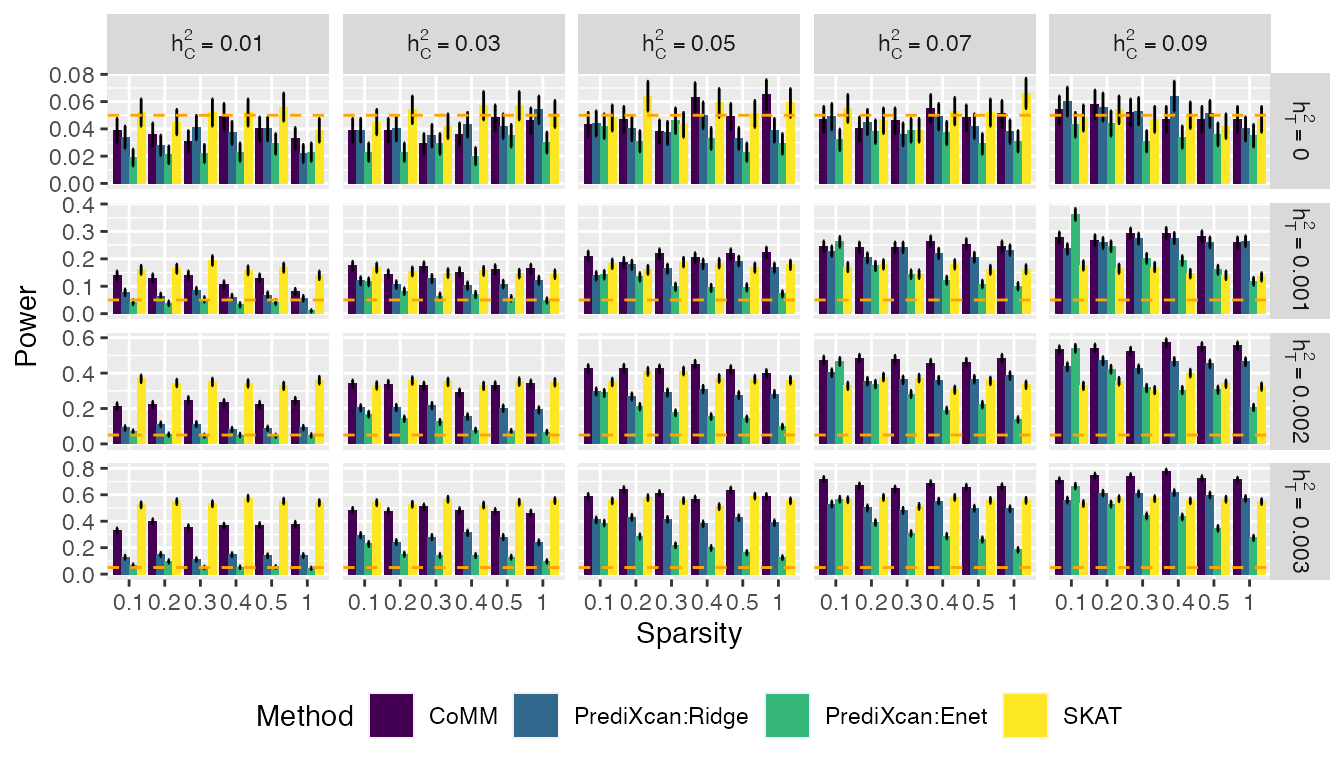
\includegraphics{CoMM_files/figure-latex/unnamed-chunk-11-1.pdf}

\subsubsection{Corrections for CoMMs (Yang et
al.)}\label{corrections-for-comms-yang-et-al.}

In Algorithm 1 (in the supplementary document), the Reduction-step
should be
\(\left( \sigma_u^{(t+1)}\right)^2 = \left( \gamma^{(t+1)}\right)^2\left( \sigma_u^{(t+1)}\right)^2\).

\subsubsection{Fit CoMM\_S2 using simulated
data}\label{fit-comm_s2-using-simulated-data}

We first generate genotype data using function \emph{genRawGeno}:

\begin{Shaded}
\begin{Highlighting}[]
\KeywordTok{library}\NormalTok{(mvtnorm)}
\KeywordTok{set.seed}\NormalTok{(}\DecValTok{1000}\NormalTok{)}
\NormalTok{L =}\StringTok{ }\DecValTok{1}\NormalTok{; M =}\StringTok{ }\DecValTok{100}\NormalTok{; rho =}\FloatTok{0.5}
\NormalTok{n1 =}\StringTok{ }\DecValTok{400}\NormalTok{; n2 =}\StringTok{ }\DecValTok{5000}\NormalTok{; n3 =}\StringTok{ }\DecValTok{400}\NormalTok{;}
\NormalTok{maf =}\StringTok{ }\KeywordTok{runif}\NormalTok{(M, }\DataTypeTok{min =} \FloatTok{0.05}\NormalTok{, }\DataTypeTok{max =} \FloatTok{0.5}\NormalTok{);}
\NormalTok{X =}\StringTok{ }\KeywordTok{genRawGeno}\NormalTok{(maf, L, M, rho, n1 }\OperatorTok{+}\StringTok{ }\NormalTok{n2);}
\NormalTok{X3 =}\StringTok{ }\KeywordTok{genRawGeno}\NormalTok{(maf, L, M, rho, n3)}
\end{Highlighting}
\end{Shaded}

Then, effect sizes are generated from standard Gaussian distribution
with sparse structure:

\begin{Shaded}
\begin{Highlighting}[]
\NormalTok{beta_prop =}\StringTok{ }\FloatTok{0.2}\NormalTok{;}
\NormalTok{b =}\StringTok{ }\KeywordTok{numeric}\NormalTok{(M);}
\NormalTok{m =}\StringTok{ }\NormalTok{M }\OperatorTok{*}\StringTok{ }\NormalTok{beta_prop;}
\NormalTok{b[}\KeywordTok{sample}\NormalTok{(M,m)] =}\StringTok{ }\KeywordTok{rnorm}\NormalTok{(m);}
\end{Highlighting}
\end{Shaded}

Subsequently, the gene expression \texttt{y} is generated by controlling
cellular heritability at prespecified level (\texttt{h2y}):

\begin{Shaded}
\begin{Highlighting}[]
\NormalTok{h2y =}\StringTok{ }\FloatTok{0.05}\NormalTok{;}
\NormalTok{b0 =}\StringTok{ }\DecValTok{6}\NormalTok{;}
\NormalTok{y0 <-}\StringTok{ }\NormalTok{X}\OperatorTok\NormalTok{b }\OperatorTok{+}\StringTok{ }\NormalTok{b0;}
\NormalTok{y  <-}\StringTok{ }\NormalTok{y0 }\OperatorTok{+}\StringTok{ }\NormalTok{(}\KeywordTok{as.vector}\NormalTok{(}\KeywordTok{var}\NormalTok{(y0)}\OperatorTok{*}\NormalTok{(}\DecValTok{1}\OperatorTok{-}\NormalTok{h2y)}\OperatorTok{/}\NormalTok{h2y))}\OperatorTok{^}\FloatTok{0.5}\OperatorTok{*}\KeywordTok{rnorm}\NormalTok{(n1}\OperatorTok{+}\NormalTok{n2);}
\end{Highlighting}
\end{Shaded}

Finally, the phenotype data is generated as the generative model of CoMM
with a prespecified trait heritability (\texttt{h2}) as:

\begin{Shaded}
\begin{Highlighting}[]
\NormalTok{h2 =}\StringTok{ }\FloatTok{0.001}\NormalTok{;}
\NormalTok{y1 <-}\StringTok{ }\NormalTok{y[}\DecValTok{1}\OperatorTok{:}\NormalTok{n1]}
\NormalTok{X1 <-}\StringTok{ }\NormalTok{X[}\DecValTok{1}\OperatorTok{:}\NormalTok{n1,]}
\NormalTok{y2 <-}\StringTok{ }\NormalTok{y0[(n1}\OperatorTok{+}\DecValTok{1}\NormalTok{)}\OperatorTok{:}\NormalTok{(n1}\OperatorTok{+}\NormalTok{n2)]}
\NormalTok{X2 <-}\StringTok{ }\NormalTok{X[(n1}\OperatorTok{+}\DecValTok{1}\NormalTok{)}\OperatorTok{:}\NormalTok{(n1}\OperatorTok{+}\NormalTok{n2),]}
\NormalTok{alpha0 <-}\StringTok{ }\DecValTok{3}  
\NormalTok{alpha <-}\StringTok{ }\FloatTok{0.3}
\NormalTok{sz2 <-}\StringTok{ }\KeywordTok{var}\NormalTok{(y2}\OperatorTok{*}\NormalTok{alpha) }\OperatorTok{*}\StringTok{ }\NormalTok{((}\DecValTok{1}\OperatorTok{-}\NormalTok{h2)}\OperatorTok{/}\NormalTok{h2)}
\NormalTok{z <-}\StringTok{ }\NormalTok{alpha0 }\OperatorTok{+}\StringTok{ }\NormalTok{y2}\OperatorTok{*}\NormalTok{alpha }\OperatorTok{+}\StringTok{ }\KeywordTok{rnorm}\NormalTok{(n2,}\DecValTok{0}\NormalTok{,}\KeywordTok{sqrt}\NormalTok{(sz2))}
\end{Highlighting}
\end{Shaded}

The genotype data \texttt{X1}, \texttt{X2} and \texttt{X3} are centered
as

\begin{Shaded}
\begin{Highlighting}[]
\NormalTok{y =}\StringTok{ }\NormalTok{y1;}
\NormalTok{mean.x1 =}\StringTok{ }\KeywordTok{apply}\NormalTok{(X1,}\DecValTok{2}\NormalTok{,mean);}
\NormalTok{x1p =}\StringTok{ }\KeywordTok{sweep}\NormalTok{(X1,}\DecValTok{2}\NormalTok{,mean.x1);}

\NormalTok{mean.x2 =}\StringTok{ }\KeywordTok{apply}\NormalTok{(X2,}\DecValTok{2}\NormalTok{,mean);}
\NormalTok{x2p =}\StringTok{ }\KeywordTok{sweep}\NormalTok{(X2,}\DecValTok{2}\NormalTok{,mean.x2);}

\NormalTok{mean.x3 =}\StringTok{ }\KeywordTok{apply}\NormalTok{(X3,}\DecValTok{2}\NormalTok{,mean);}
\NormalTok{x3p =}\StringTok{ }\KeywordTok{sweep}\NormalTok{(X3,}\DecValTok{2}\NormalTok{,mean.x3);}

\NormalTok{w =}\StringTok{ }\KeywordTok{matrix}\NormalTok{(}\KeywordTok{rep}\NormalTok{(}\DecValTok{1}\NormalTok{,n1),}\DataTypeTok{ncol=}\DecValTok{1}\NormalTok{);}
\end{Highlighting}
\end{Shaded}

The summary statistics are generated from GWAS individual data

\begin{Shaded}
\begin{Highlighting}[]
\NormalTok{hatmu =}\StringTok{ }\KeywordTok{matrix}\NormalTok{(}\DecValTok{0}\NormalTok{, M, }\DecValTok{1}\NormalTok{)}
\NormalTok{hats =}\StringTok{ }\KeywordTok{matrix}\NormalTok{(}\DecValTok{0}\NormalTok{, M, }\DecValTok{1}\NormalTok{)}

\ControlFlowTok{for}\NormalTok{ (m }\ControlFlowTok{in} \DecValTok{1}\OperatorTok{:}\NormalTok{M)\{}
\NormalTok{  fm =}\StringTok{ }\KeywordTok{lm}\NormalTok{(z}\OperatorTok{~}\DecValTok{1}\OperatorTok{+}\NormalTok{x2p[,m]);}
\NormalTok{  hatmu[m] =}\StringTok{ }\KeywordTok{summary}\NormalTok{(fm)}\OperatorTok{$}\NormalTok{coefficients[}\DecValTok{2}\NormalTok{,}\DecValTok{1}\NormalTok{]}
\NormalTok{  hats[m] =}\StringTok{ }\KeywordTok{summary}\NormalTok{(fm)}\OperatorTok{$}\NormalTok{coefficients[}\DecValTok{2}\NormalTok{,}\DecValTok{2}\NormalTok{];}
\NormalTok{\}}
\end{Highlighting}
\end{Shaded}

The correlation matrix reflecting LD information is estimated using
reference panel

\begin{Shaded}
\begin{Highlighting}[]
\NormalTok{lam =}\StringTok{ }\FloatTok{0.8}
\NormalTok{sumx3p =}\StringTok{ }\KeywordTok{apply}\NormalTok{(x3p}\OperatorTok{*}\NormalTok{x3p, }\DecValTok{2}\NormalTok{, sum)}
\NormalTok{R =}\StringTok{ }\KeywordTok{matrix}\NormalTok{(}\DecValTok{0}\NormalTok{, M, M);}
\ControlFlowTok{for}\NormalTok{ (i1 }\ControlFlowTok{in} \DecValTok{1}\OperatorTok{:}\NormalTok{M)\{}
  \ControlFlowTok{for}\NormalTok{ (j1 }\ControlFlowTok{in} \DecValTok{1}\OperatorTok{:}\NormalTok{M)\{}
\NormalTok{    R[i1,j1] =}\StringTok{ }\KeywordTok{t}\NormalTok{(x3p[,i1])}\OperatorTok\NormalTok{x3p[,j1]}\OperatorTok{/}\KeywordTok{sqrt}\NormalTok{(sumx3p[i1]}\OperatorTok{*}\NormalTok{sumx3p[j1])                        }
\NormalTok{  \}}
\NormalTok{\}}
\NormalTok{R =}\StringTok{ }\NormalTok{R}\OperatorTok{*}\NormalTok{lam }\OperatorTok{+}\StringTok{ }\NormalTok{(}\DecValTok{1} \OperatorTok{-}\StringTok{ }\NormalTok{lam)}\OperatorTok{*}\KeywordTok{diag}\NormalTok{(M)  }
\end{Highlighting}
\end{Shaded}

The likelihood ratio test is implemented

\begin{Shaded}
\begin{Highlighting}[]
\NormalTok{px =}\StringTok{ }\DecValTok{1}
\NormalTok{opts =}\StringTok{ }\KeywordTok{list}\NormalTok{(}\DataTypeTok{max_iter =} \DecValTok{10000}\NormalTok{, }\DataTypeTok{dispF =} \DecValTok{1}\NormalTok{, }\DataTypeTok{display_gap =} \DecValTok{10}\NormalTok{, }\DataTypeTok{epsStopLogLik =} \FloatTok{1e-5}\NormalTok{, }\DataTypeTok{fix_alphag =} \DecValTok{0}\NormalTok{);}
\NormalTok{opts1 =}\StringTok{ }\KeywordTok{list}\NormalTok{(}\DataTypeTok{max_iter =} \DecValTok{10000}\NormalTok{, }\DataTypeTok{dispF =} \DecValTok{1}\NormalTok{, }\DataTypeTok{display_gap =} \DecValTok{10}\NormalTok{, }\DataTypeTok{epsStopLogLik =} \FloatTok{1e-5}\NormalTok{, }\DataTypeTok{fix_alphag =} \DecValTok{1}\NormalTok{);}

\NormalTok{fmHa =}\StringTok{ }\KeywordTok{CoMM_S2}\NormalTok{(x1p, y, w, hatmu, hats, R, opts, px);}
\CommentTok{#> ***Iteration*******Fnew********Fold**********Diff***}
\CommentTok{#>   1.0000e+001 -1.1934e+003 -1.1934e+003  1.3005e-002}
\NormalTok{fmH0 =}\StringTok{ }\KeywordTok{CoMM_S2}\NormalTok{(x1p, y, w, hatmu, hats, R, opts1, px);}
\CommentTok{#> ***Iteration*******Fnew********Fold**********Diff***}
\CommentTok{#>   1.0000e+001 -1.1989e+003 -1.1989e+003  1.6075e-003}

\NormalTok{stat =}\StringTok{ }\DecValTok{2}\OperatorTok{*}\NormalTok{(fmHa}\OperatorTok{$}\NormalTok{LRLB }\OperatorTok{-}\StringTok{ }\NormalTok{fmH0}\OperatorTok{$}\NormalTok{LRLB)}
\NormalTok{pval =}\StringTok{ }\KeywordTok{pchisq}\NormalTok{(stat, }\DecValTok{1}\NormalTok{, }\DataTypeTok{lower.tail =}\NormalTok{ F)}
\KeywordTok{str}\NormalTok{(fmHa)}
\CommentTok{#> List of 7}
\CommentTok{#>  $ vardist_mu: num [1:100, 1] -0.1061 -0.1586 -0.0563 -0.08 -0.2769 ...}
\CommentTok{#>  $ sigma2mu  : num 0.2}
\CommentTok{#>  $ alphag    : num 0.749}
\CommentTok{#>  $ sigma2beta: num 0.329}
\CommentTok{#>  $ sigma2y   : num 105}
\CommentTok{#>  $ LRLB      : num -1276}
\CommentTok{#>  $ Lq        : num [1, 1:19] -1375 -1203 -1197 -1195 -1194 ...}
\KeywordTok{str}\NormalTok{(fmH0)}
\CommentTok{#> List of 7}
\CommentTok{#>  $ vardist_mu: num [1:100, 1] -0.6199 0.0629 -0.0129 0.1128 -0.2567 ...}
\CommentTok{#>  $ sigma2mu  : num 0.221}
\CommentTok{#>  $ alphag    : num 0}
\CommentTok{#>  $ sigma2beta: num 0.329}
\CommentTok{#>  $ sigma2y   : num 105}
\CommentTok{#>  $ LRLB      : num -1282}
\CommentTok{#>  $ Lq        : num [1, 1:16] -1377 -1206 -1201 -1199 -1199 ...}
\KeywordTok{print}\NormalTok{(stat)}
\CommentTok{#> [1] 11.9037}
\KeywordTok{print}\NormalTok{(pval)}
\CommentTok{#> [1] 0.0005602251}
\end{Highlighting}
\end{Shaded}

The output of CoMM\_S2 is a list with 7 variables, mean of variational
distribution \texttt{vardist\_mu}, variance component \texttt{sigma2mu},
gene effect size \texttt{alphag}, variance component \texttt{sigma2y},
calibariated ELBO \texttt{LRLB}, original ELBO \texttt{Lq}.

\subsubsection{Fit CoMM\_S2 using GWAS and eQTL
data}\label{fit-comm_s2-using-gwas-and-eqtl-data}

The example of running CoMM\_S2 using GWAS summary statistics and eQTL
data in plink binary format

\begin{Shaded}
\begin{Highlighting}[]
\NormalTok{file1 =}\StringTok{ "1000G.EUR.QC.1"}\NormalTok{;}
\NormalTok{file2 =}\StringTok{ "NFBC_beta_se_TG.txt"}
\NormalTok{file3 =}\StringTok{ "Geuvadis_gene_expression_qn.txt"}\NormalTok{;}
\NormalTok{file4 =}\StringTok{ "1000G_chr_all"}\NormalTok{;}
\NormalTok{file5 =}\StringTok{ ""}\NormalTok{;}
\NormalTok{bw =}\StringTok{ }\DecValTok{500000}\NormalTok{;}
\NormalTok{lam =}\StringTok{ }\FloatTok{0.95}\NormalTok{;}
\NormalTok{coreNum =}\StringTok{ }\DecValTok{24}\NormalTok{;}
\end{Highlighting}
\end{Shaded}

Here, file1 is the prefix for eQTL genotype data in plink binary format,
file2 is the GWAS summary data, file3 is the prefix for reference panel
data in plink binary format, file4 is the gene expression file with
extended name, file5 are covariates file for eQTL data. bw is the number
of downstream and upstream SNPs that are considered as cis-SNP within a
gene. lam is the shirnkage intensify for reference panel. coreNum is the
number of cores in parallel. Then run
\texttt{fm\ =\ CoMM\_S2\_testing(file1,\ file2,\ file3,\ file4,\ file5,\ bw,\ lam);}.
For GWAS summary data file, it must have the following format (note that
it must be tab delimited):

\begin{longtable}[]{@{}lrrllrr@{}}
\toprule
SNP & chr & BP & A1 & A2 & beta & se\tabularnewline
\midrule
\endhead
rs3094315 & 1 & 752566 & G & A & -0.0122 & 0.0294\tabularnewline
rs3128117 & 1 & 944564 & C & T & -0.0208 & 0.0278\tabularnewline
rs1891906 & 1 & 950243 & C & A & -0.0264 & 0.0260\tabularnewline
rs2710888 & 1 & 959842 & T & C & -0.0439 & 0.0297\tabularnewline
rs4970393 & 1 & 962606 & G & A & -0.0252 & 0.0233\tabularnewline
rs7526076 & 1 & 998395 & A & G & -0.0512 & 0.0229\tabularnewline
rs4075116 & 1 & 1003629 & C & T & -0.0497 & 0.0220\tabularnewline
rs3934834 & 1 & 1005806 & T & C & 0.0364 & 0.0256\tabularnewline
rs3766192 & 1 & 1017197 & C & T & -0.0116 & 0.0178\tabularnewline
rs3766191 & 1 & 1017587 & T & C & 0.0318 & 0.0262\tabularnewline
\bottomrule
\end{longtable}

To make `CoMM\_S2' further speeding, we implement multiple thread
version of `CoMM\_S2' by just run
\texttt{fm\ =\ CoMM\_S2\_paral\_testing(file1,\ file2,\ file3,\ file4,\ file5,\ bw,\ lam,\ coreNum);}

\subsubsection{Figures}\label{figures-1}

The following data and codes are used to produce the barplot of power

\begin{Shaded}
\begin{Highlighting}[]
\KeywordTok{library}\NormalTok{(ggplot2)}
\KeywordTok{library}\NormalTok{(colorspace)}
\NormalTok{bp2 <-}\StringTok{ }\KeywordTok{ggplot}\NormalTok{(pval2, }\KeywordTok{aes}\NormalTok{(}\DataTypeTok{x=}\NormalTok{Sparsity, }\DataTypeTok{y=}\NormalTok{Power, }\DataTypeTok{fill=}\NormalTok{Method)) }\OperatorTok{+}
\StringTok{    }\KeywordTok{geom_bar}\NormalTok{(}\DataTypeTok{stat=}\StringTok{"identity"}\NormalTok{, }\DataTypeTok{position=}\KeywordTok{position_dodge}\NormalTok{()) }\OperatorTok{+}\StringTok{ }
\StringTok{    }\KeywordTok{facet_grid}\NormalTok{(h2}\OperatorTok{~}\NormalTok{hc, }\DataTypeTok{scales =} \StringTok{"free"}\NormalTok{, }\DataTypeTok{labeller =}\NormalTok{ label_parsed)  }\OperatorTok{+}
\StringTok{    }\KeywordTok{theme}\NormalTok{(}\DataTypeTok{strip.text.x =} \KeywordTok{element_text}\NormalTok{(}\DataTypeTok{size=}\DecValTok{12}\NormalTok{, }\DataTypeTok{color=}\StringTok{"black"}\NormalTok{,}
                                      \DataTypeTok{face=}\StringTok{"bold"}\NormalTok{),}
          \DataTypeTok{strip.text.y =} \KeywordTok{element_text}\NormalTok{(}\DataTypeTok{size=}\DecValTok{12}\NormalTok{, }\DataTypeTok{color=}\StringTok{"black"}\NormalTok{,}
                                      \DataTypeTok{face=}\StringTok{"bold"}\NormalTok{),}
          \DataTypeTok{plot.title =} \KeywordTok{element_text}\NormalTok{(}\DataTypeTok{size=}\DecValTok{20}\NormalTok{,}\DataTypeTok{face =} \StringTok{"bold"}\NormalTok{,}\DataTypeTok{hjust=}\FloatTok{0.5}\NormalTok{),}
          \DataTypeTok{axis.title.x =} \KeywordTok{element_text}\NormalTok{(}\DataTypeTok{size=}\DecValTok{8}\NormalTok{,}\DataTypeTok{face =} \StringTok{"bold"}\NormalTok{),}
          \DataTypeTok{axis.text.x =} \KeywordTok{element_text}\NormalTok{(}\DataTypeTok{size=}\DecValTok{8}\NormalTok{,}\DataTypeTok{face =} \StringTok{"bold"}\NormalTok{),}
          \DataTypeTok{axis.title.y =} \KeywordTok{element_blank}\NormalTok{(),}
          \DataTypeTok{axis.text.y =} \KeywordTok{element_text}\NormalTok{(}\DataTypeTok{size=}\DecValTok{15}\NormalTok{,}\DataTypeTok{face =} \StringTok{"bold"}\NormalTok{),}
          \DataTypeTok{legend.position=}\StringTok{"bottom"}\NormalTok{,}
          \DataTypeTok{legend.title=}\KeywordTok{element_text}\NormalTok{(}\DataTypeTok{size=}\DecValTok{15}\NormalTok{),}
          \DataTypeTok{legend.text=}\KeywordTok{element_text}\NormalTok{(}\DataTypeTok{size=}\DecValTok{15}\NormalTok{))}
\NormalTok{  colours<-}\KeywordTok{rainbow_hcl}\NormalTok{(}\DecValTok{3}\NormalTok{, }\DataTypeTok{start =} \DecValTok{0}\NormalTok{, }\DataTypeTok{end =} \DecValTok{300}\NormalTok{)}
\NormalTok{  bp2 =}\StringTok{ }\NormalTok{bp2 }\OperatorTok{+}\StringTok{ }\KeywordTok{scale_fill_manual}\NormalTok{(}\DataTypeTok{values=}\NormalTok{colours, }\DataTypeTok{labels=}\KeywordTok{expression}\NormalTok{(}\StringTok{"CoMM-S"}\OperatorTok{^}\DecValTok{2}\NormalTok{,}\StringTok{"S-PrediXcan:Ridge"}\NormalTok{,}\StringTok{"S-PrediXcan:Enet"}\NormalTok{))}
\NormalTok{bp2}
\end{Highlighting}
\end{Shaded}

\begin{center}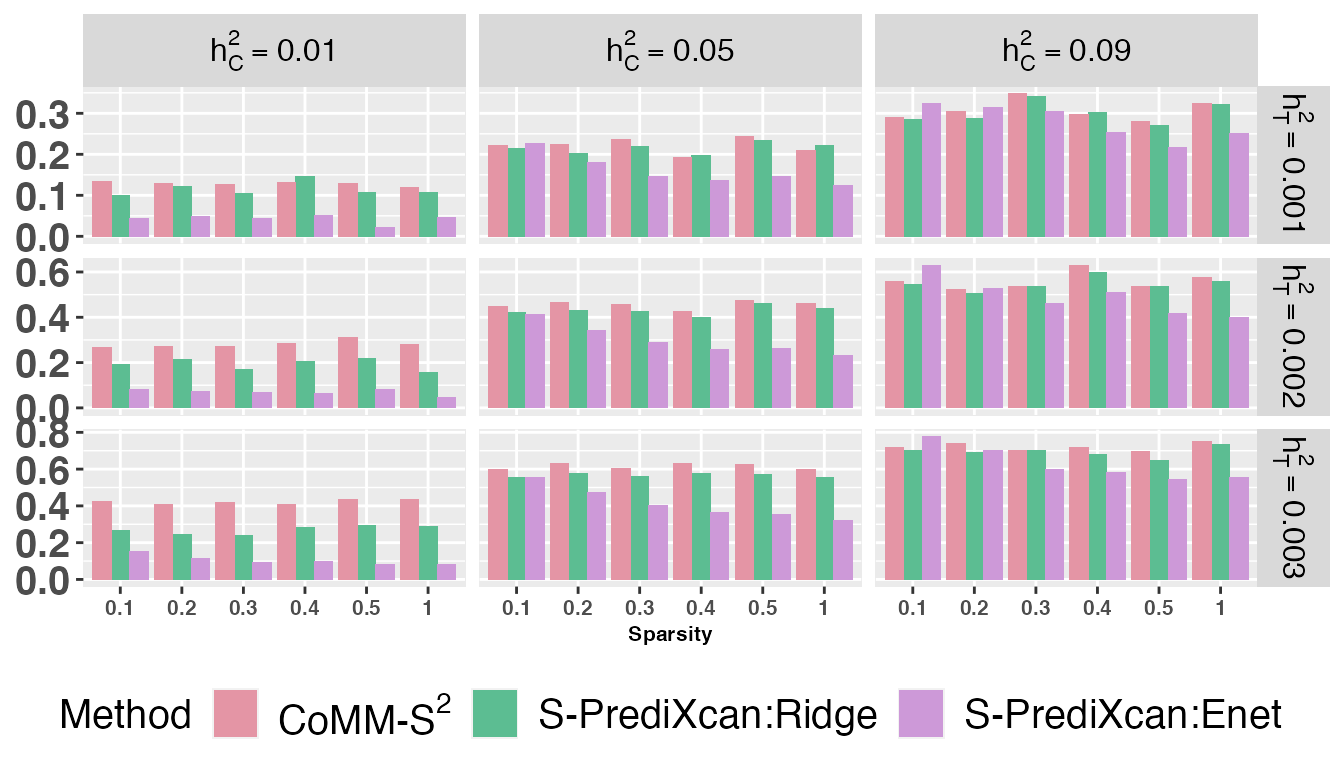
\includegraphics{CoMM_files/figure-latex/unnamed-chunk-22-1} \end{center}


\end{document}
